\chapter{Transparency in healthcare}

\section{Methods}

With these evidences of healthcare information needs, we developed Healthcare
Network, a web application that lists every hospital in France, and displays key
statistics on them. The application is directed to either health professionals
or patients. Health professionals might use it to gain insights about specific
hospitals, and look for the best place to send their patients when they lack
expertise. Patients could learn more about the hospital they have been sent to,
check the care quality or surgery volume.

To create the Healthcare-Network web application, we centralized the several
datasets into databases. We then built the backend of the application with
Python and Flask framework, while the frontend was coded with HTML and CSS from
the Bootstrap library. We used two databases: a relational database (MySQL) and
a no relational database (Mongo DB). In Mongo DB, we stored the datasets to draw
the interactive maps in the application. We used the geojson format, which works
well with Mongo DB. All the other datasets are stored in the relational
database. There are roughly 40 tables in the relational database. The most used
tables are statistics on the hospitals and on the municipalities. We chose to
use the Flask framework for its simplicity and the high number of users. The
framework has a simple core to quickly build a working web application with
little code. It can be improved with extensions that add new features. With such
framework, we built several API routes that render HTML and CSS templates to the
users. The interactive maps were built with the Folium library, and the other
figures with Plotly.

\section{Results}

In this section, we will describe the most important features of the web
application, illustrated with screen captures from the website.

The landing page of the application is a minimalist search bar, as illustrated
on \cref{fig:hn-home}. The search feature lets the user look for hospitals by
name, category or location. In this first version, the search algorithm is
fairly basic and matches the hospitals that contains the text query in either
its name category or location. No weighting or additional rule was added. The
search feature could be improved later on, by using dedicated and search focused
databases like the very popular Elastic Search.

\begin{figure}[h]
    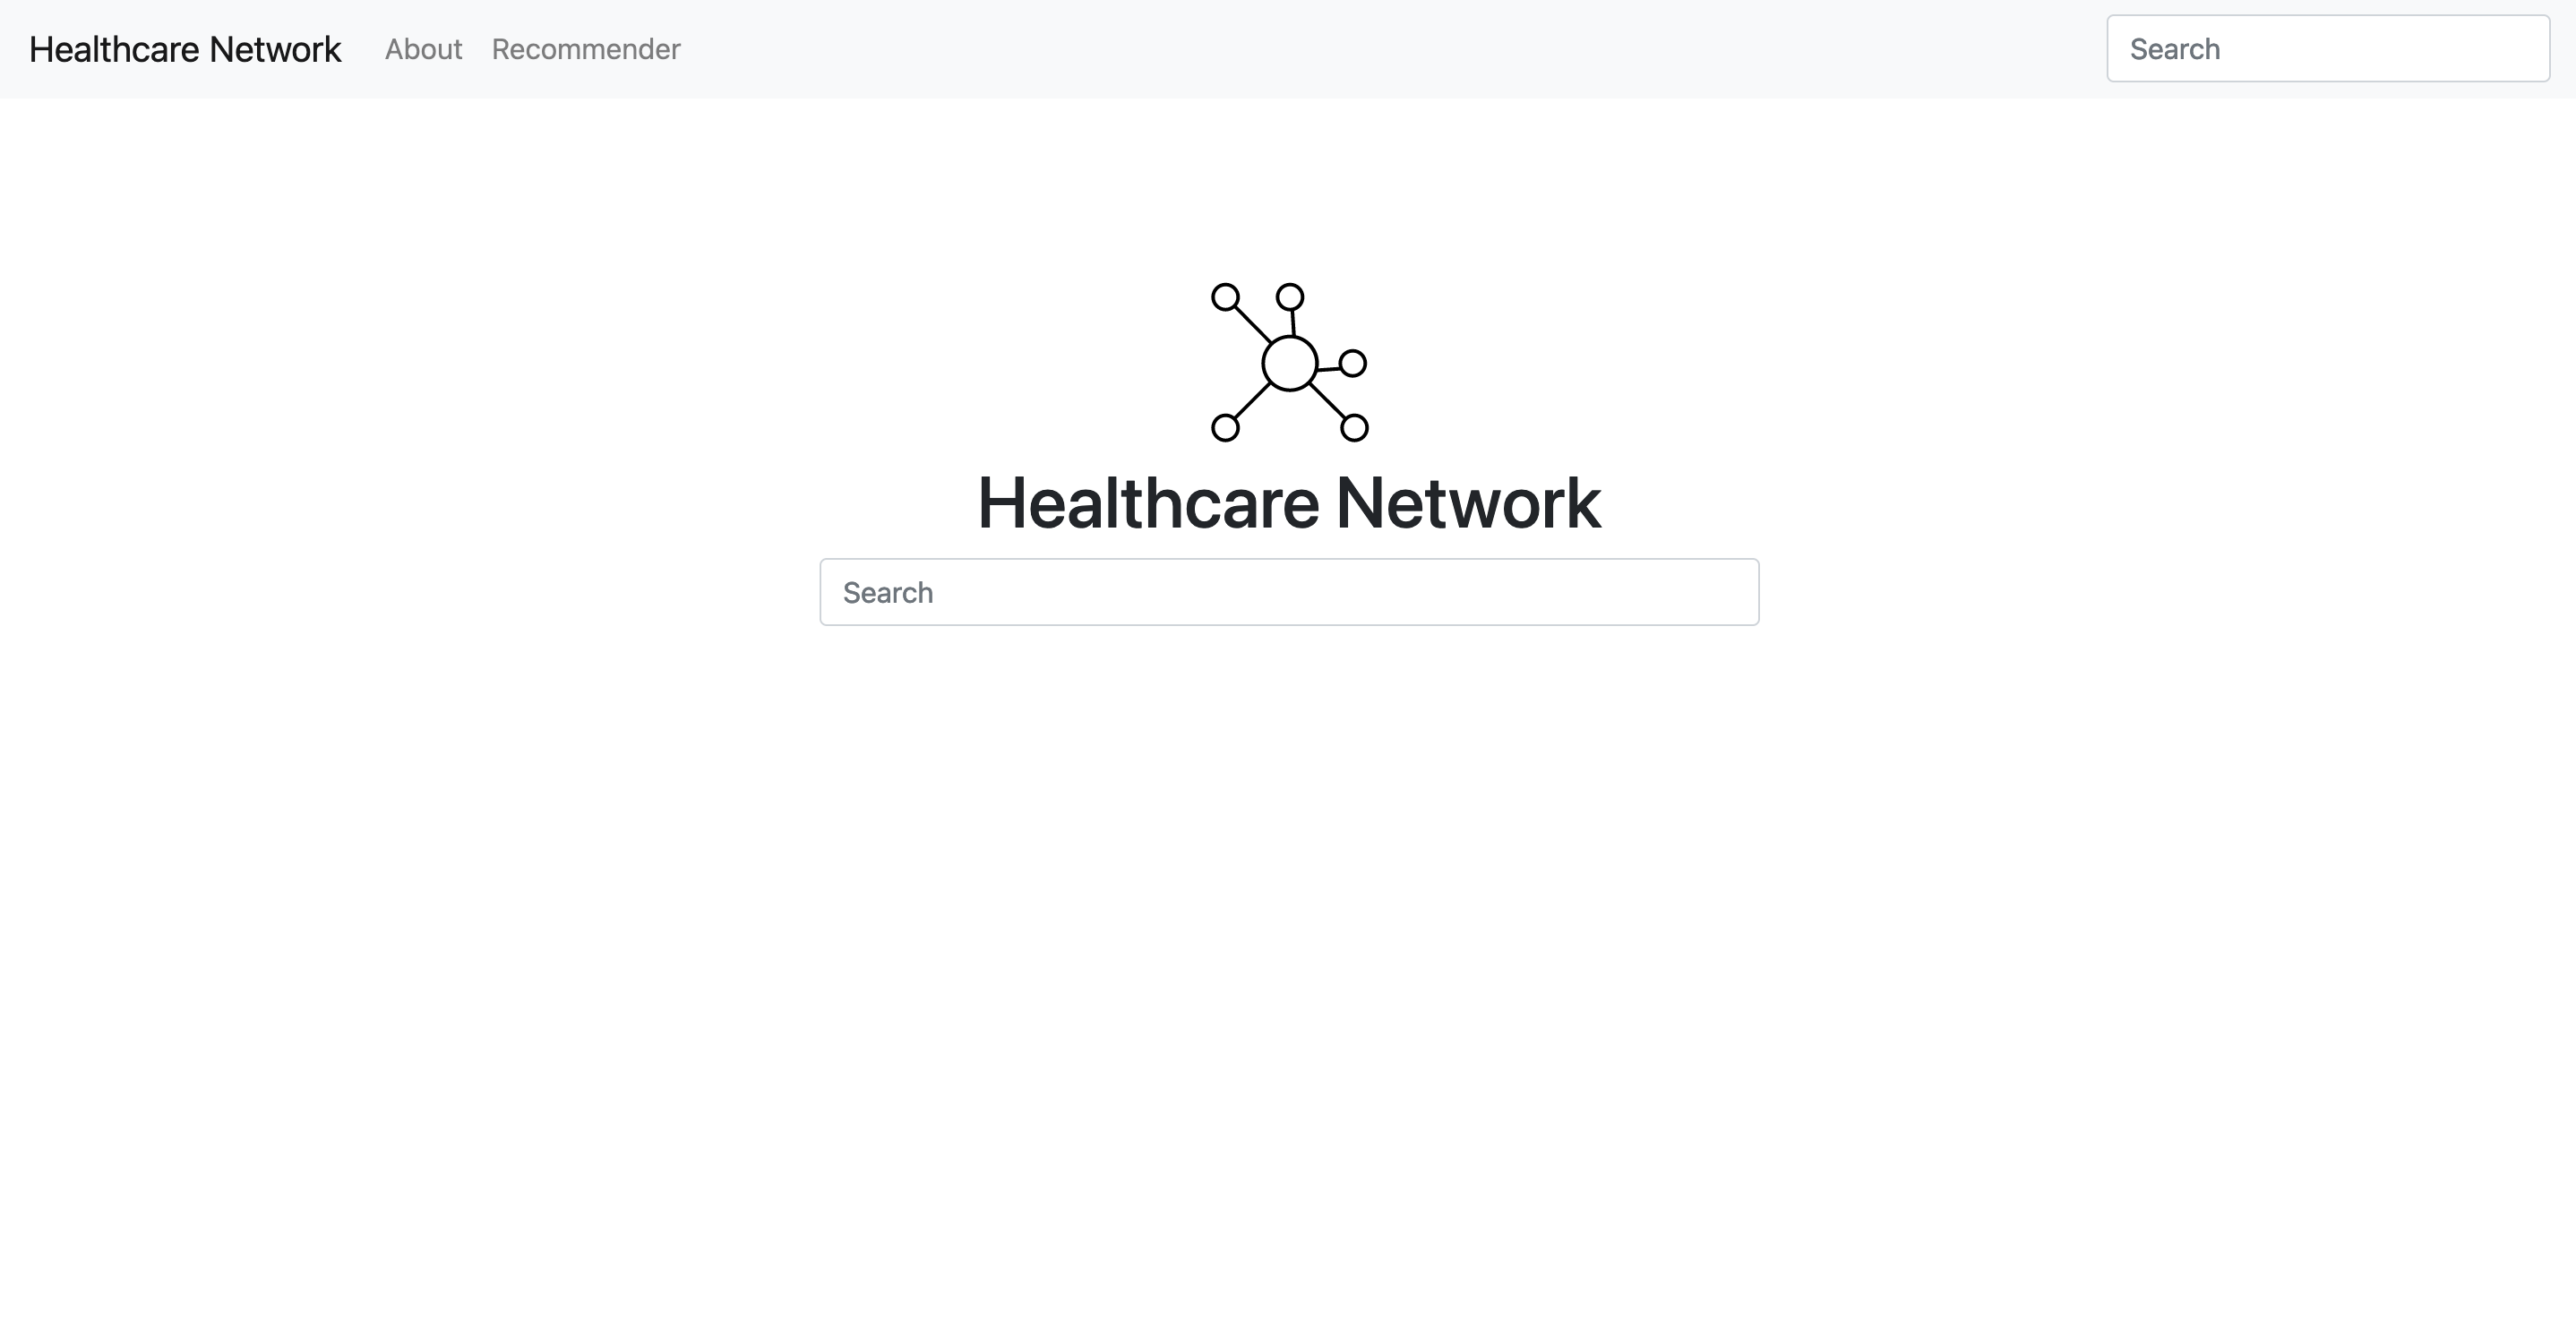
\includegraphics[width=0.7\textwidth]{images/healthcare-network/home.png}
    \centering
    \caption{ \textbf{Healthcare-Network: homepage.} A minimalist page with a
        search bar allowing to find hospitals based on their name, category, or
        location. }
    \label{fig:hn-home}
\end{figure}

We now provide a search example, and \cref{fig:hn-search} shows the results of
the query ``chu'', corresponding to the \acf{chru} hospital category. 153
results were returned, displayed as a list on the left and on a map on the right
side of the screen. The list shows basic informations about the retrieved
hospitals, including their names, locations, categories and type of care
provided, like \acf{mco} for instance. The map is interactive, and lets the user
visualize the spatial distribution of the retrieved hospitals. On the map, the
hospitals are displayed as icons, colored by hospital category. This query
illustrates an additional feature of the search bar: show the spatial distribution
of the hospitals in France by category.

\begin{figure}[h]
    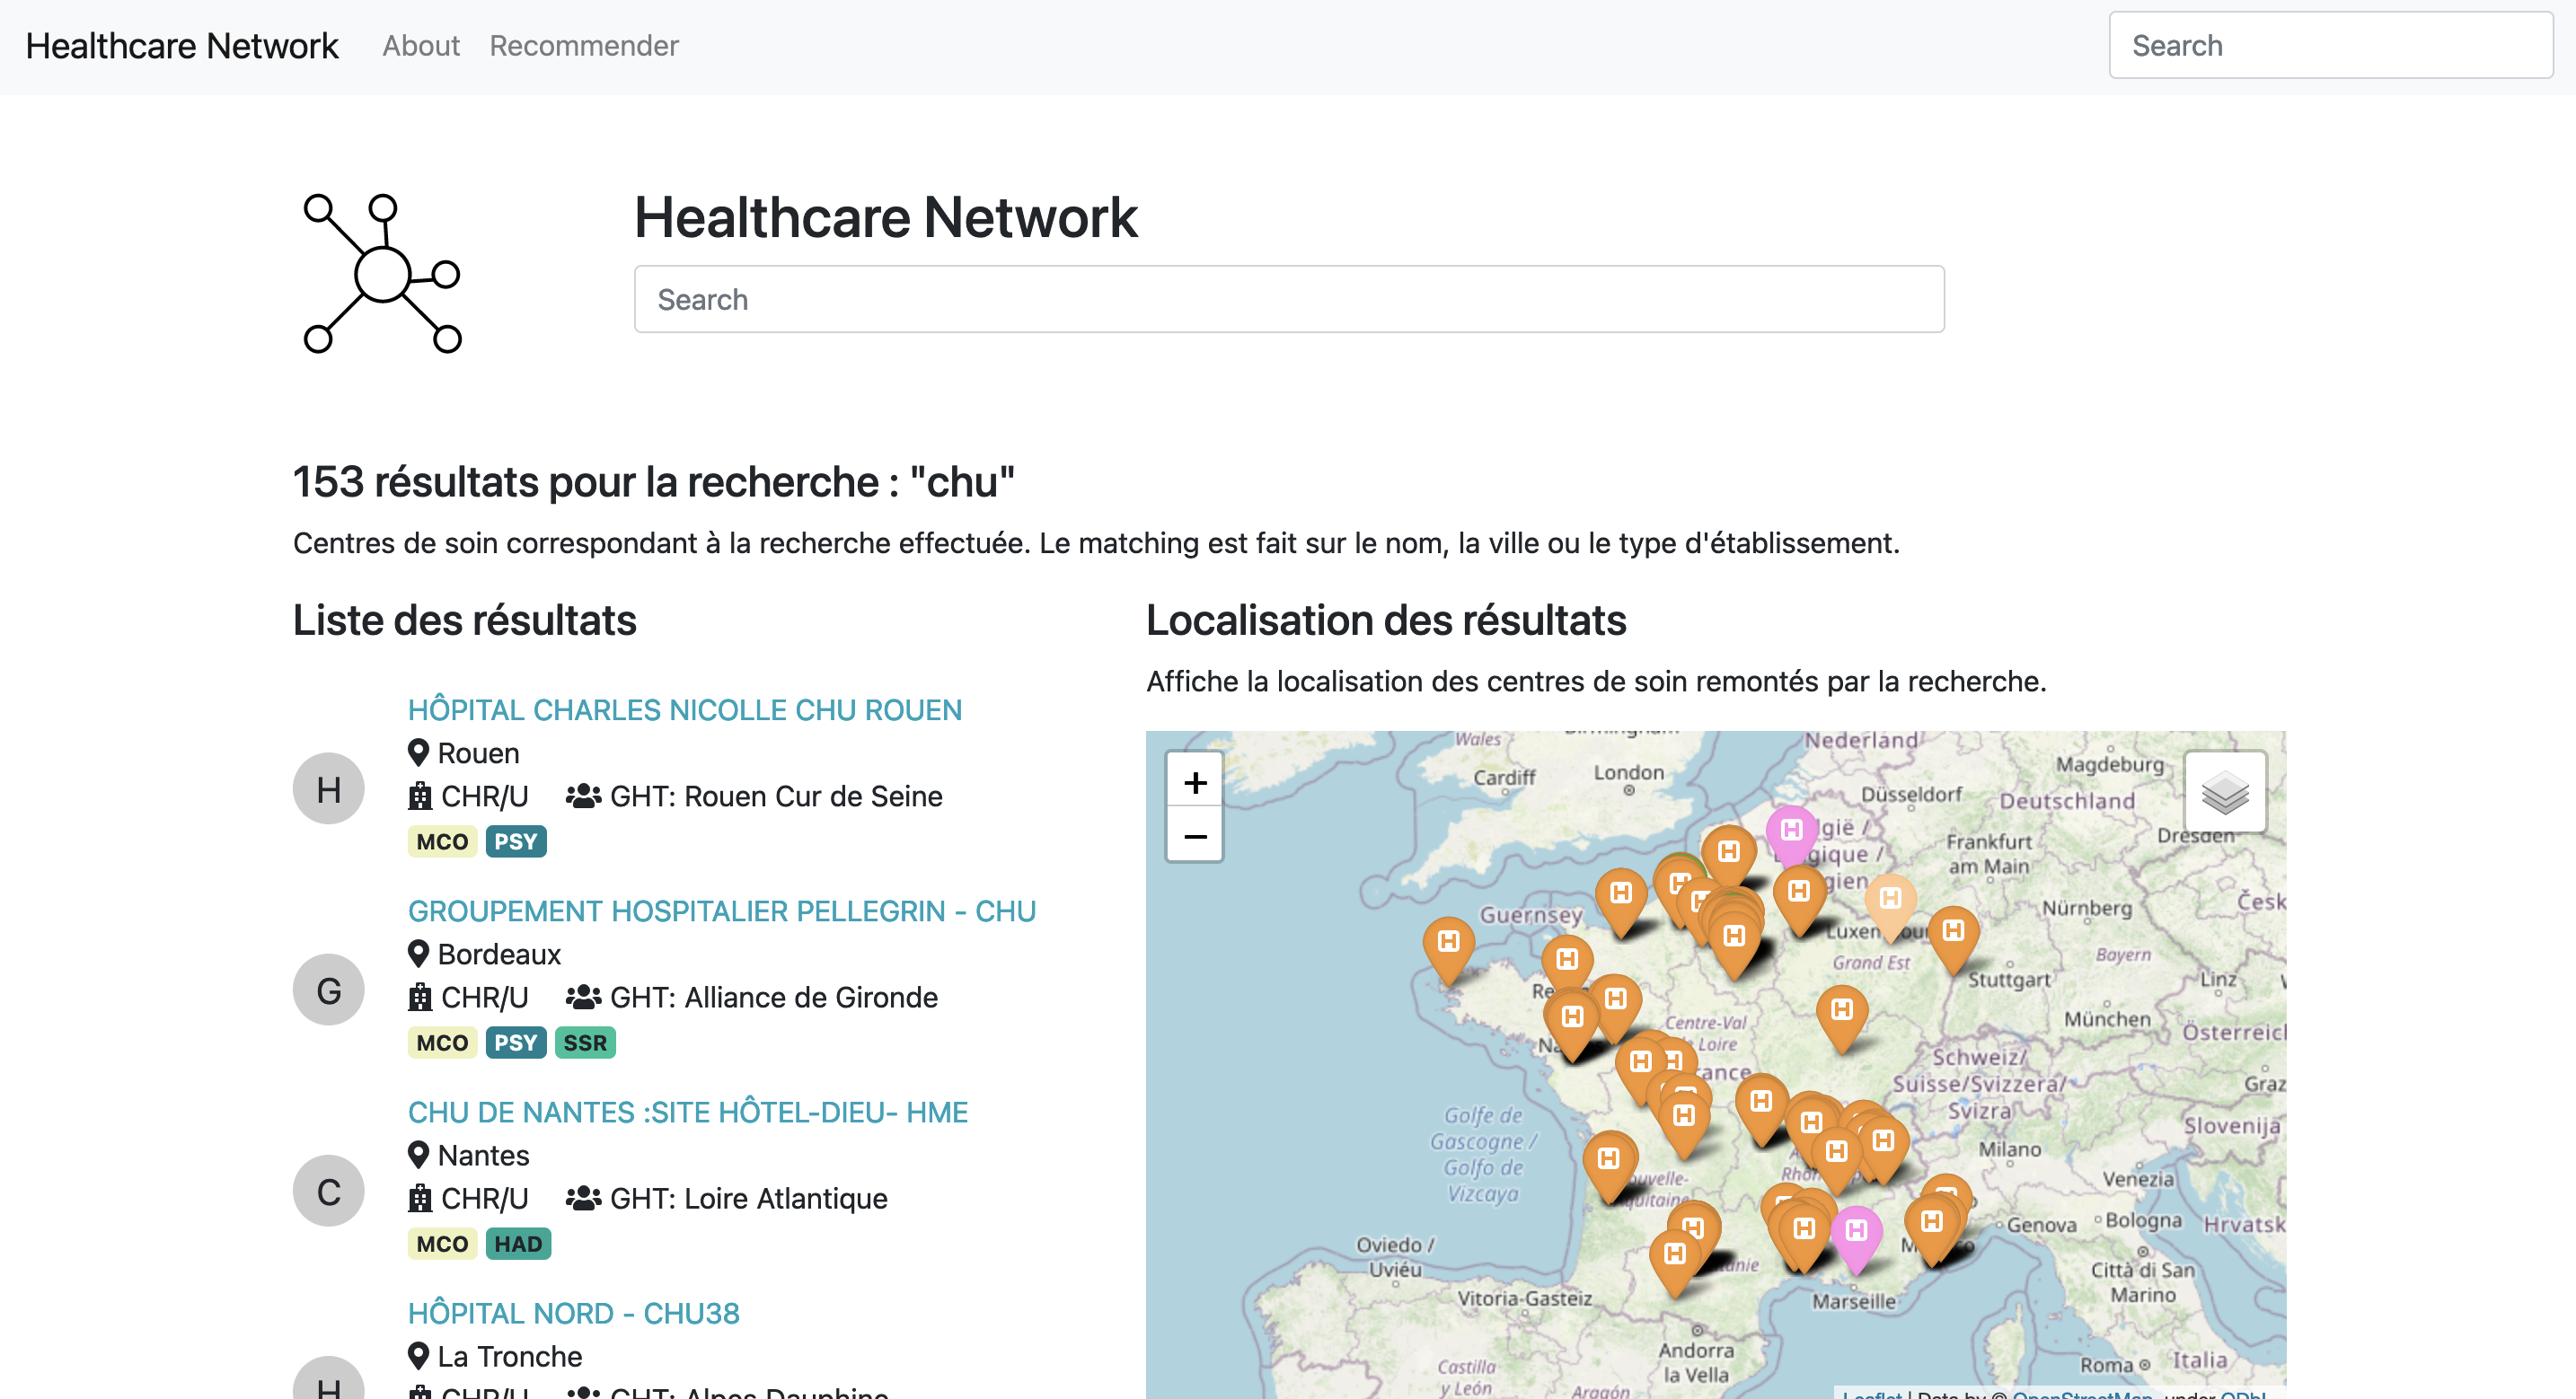
\includegraphics[width=0.7\textwidth]{images/healthcare-network/search.png}
    \centering
    \caption{ \textbf{Healthcare-Network: search results.} The list of retrieved
        hospitals and their details is displayed, as their position on a map.
        This query shows all the \ac{chru} hospitals in metropolitan France. }
    \label{fig:hn-search}
\end{figure}

Each hospital has its individual web page, as illustrated on
\cref{fig:hn-coulommiers-page} with the \ac{ch} de Coulommiers. The web page
shows basic informations about the hospital, with name, location and category
displayed first. A navigation pane also shows the hospitals from the same
\ac{ght} and legal entity. Hospitals within the same \ac{ght} share their
information system. This grouping was introduced in 2016 for the public
hospitals only. They aimed at facilitating the communication between these
facilities, and make it easier to transfer patients from one hospital to another
if needed. Hospitals from the same legal entity are governed by the same
administration, but spread among multiple geographical sites. Hospitals in large
cities such as Paris, Marseille or Lyon have most of their largest hospitals
belonging to the same legal entity. For instance in Paris, the AP-HP legal entity
gathers 39 hospitals spread across the Ile-de-France region.
The hospital location is shown on an interactive map, where the user can
zoom in and out, and add more indicators, including:

\begin{itemize}
    \item The municipalities populations and median salary. These indicators are
          a way to gain insight about the hospital neighborhood, and neighboring
          demand. To display these indicators, we color the municipality according
          to the indicator value.
    \item Patients provenance. We display the number of patients who visited
          this hospital per municipalities within a year. Through this, it is
          easy to evaluate how influent and important an hospital is, based on
          how many patients it is draining from further population locations.
          Usually, small local hospitals tend to receive patients from their
          immediate neighborhood; where large hospitals specialized in oncology
          like Institut Curie or Institut Gustave Roussy will treat patients
          from many different regions.
    \item Other hospitals from the same \ac{ght}. We display on the map the other
          hospitals that share the same information system. With this information,
          we can evaluate how close this hospital is to other hospitals where it
          would be easy to transfer patients if the desired pathology is not treated
          in this hospital.
    \item Other hospitals that shared patients with this hospital within a year.
          We call this 'co-occurrences', and a higher number shows that two
          hospitals seems to work closely together. For instance, one hospital
          might handle the cancer surgery and send their patients to another
          hospital for radiotherapy. Identifying hospitals that frequently
          exchange patients is a good way to find alternative hospitals for
          certain pathologies. There is also a high chance that these two
          hospitals communicate frequently with each other, making it easier
          to send patients and keep track of what happened in their pathways.
\end{itemize}

\begin{figure}[h]
    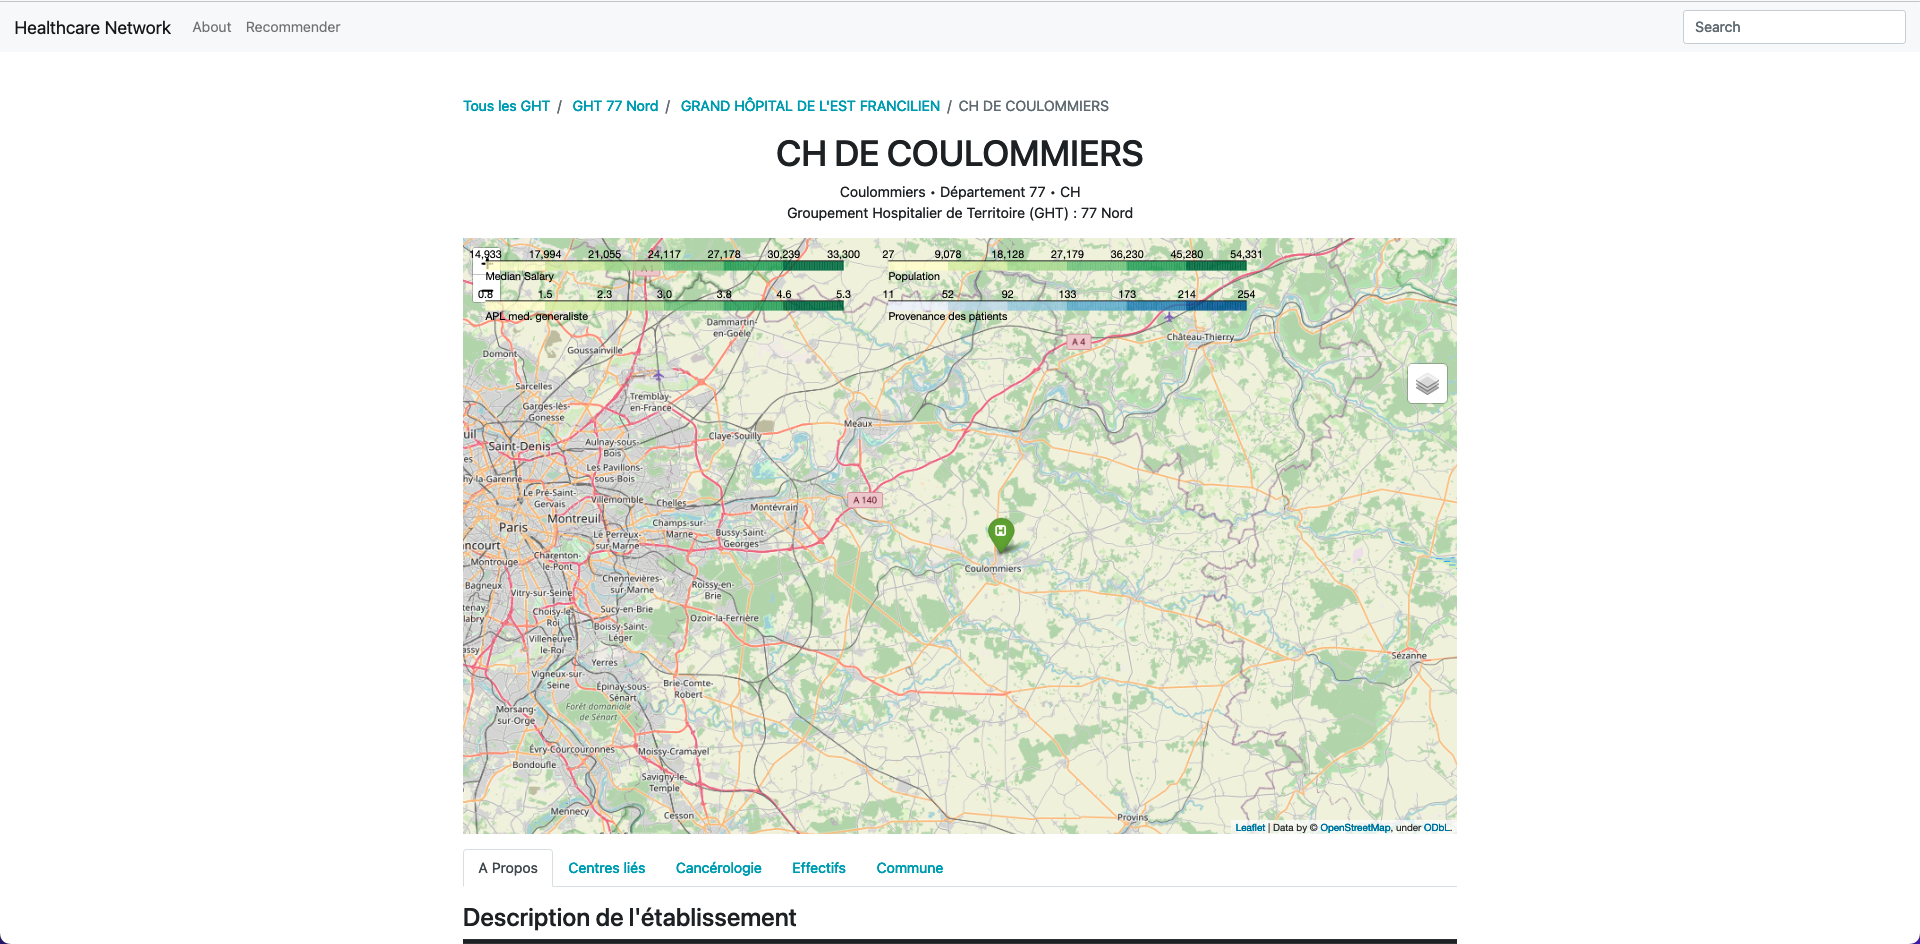
\includegraphics[width=0.7\textwidth]{images/healthcare-network/hospital-page.png}
    \centering
    \caption{ \textbf{Healthcare-Network: example of an hospital page, \acf{ch}
            de Coulommiers.} The web page shows basic informations about the
        hospital, with name, location and category displayed first. A navigation
        pane also shows the hospital \ac{ght} and legal entity. The hospital
        location is shown on an interactive map. }
    \label{fig:hn-coulommiers-page}
\end{figure}

The \cref{fig:hn-coulommiers-co-occ} is an example of the interactive map
mentioned earlier. Here, we colored the municipalities by the number of patients
who visited \ac{ch} de Coulommiers. We also displayed hospitals from the same
legal entity in green. Finally, we show hospitals that exchanged patients with
\ac{ch} de Coulommiers as blue links. From this map, we observe that \ac{ch} de
Coulommiers mostly attract patients from the neighboring municipalities. The
hospitals with the most co-occurrences are either from the same \ac{ght}, or
located in Paris. This might mean that patients with complications were sent to
larger hospitals in Paris.

\begin{figure}[h]
    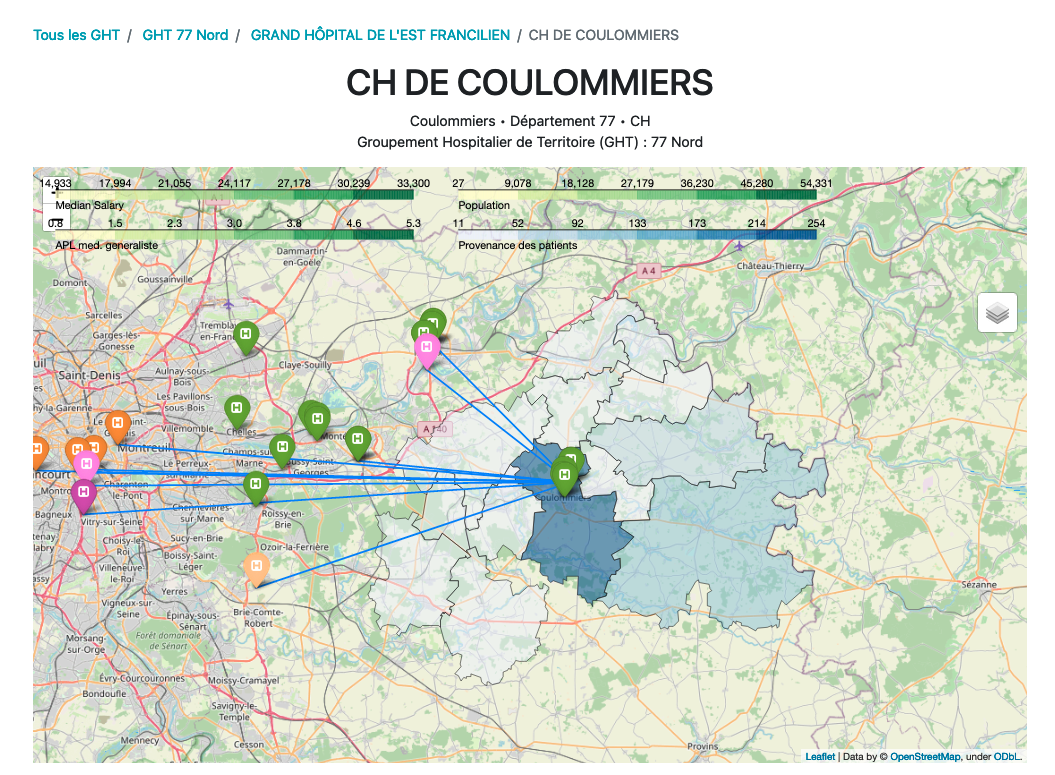
\includegraphics[width=0.7\textwidth]{images/healthcare-network/coulommiers-co-occ.png}
    \centering
    \caption{ \textbf{Healthcare-Network: example of an hospital page, \acf{ch}
            de Coulommiers.} We filled the municipalities by the number of patients
        who visited \ac{ch} de Coulommiers. We also displayed hospitals from the
        same legal entity in green. Finally, we show hospitals that exchanged
        patients with \ac{ch} de Coulommiers as blue links. }
    \label{fig:hn-coulommiers-co-occ}
\end{figure}

Below this interactive map, we display the list of services and number of
\ac{mco} stays and beds for hospitals. For instance, on
\cref{fig:hn-curie-services}, we displayed this information for the Institut
Curie Paris hospital. The list of services allows to quickly evaluate the
hospital ability to treat cancer patients. The number of stays and number of
beds lets the users evaluate the hospital size, and how saturated it is. We see
that Institut Curie has all the main services besides psychiatry and palliative
care. From the activity statistics, we see that this hospital does not do any
obstetric activity.

\begin{figure}[h]
    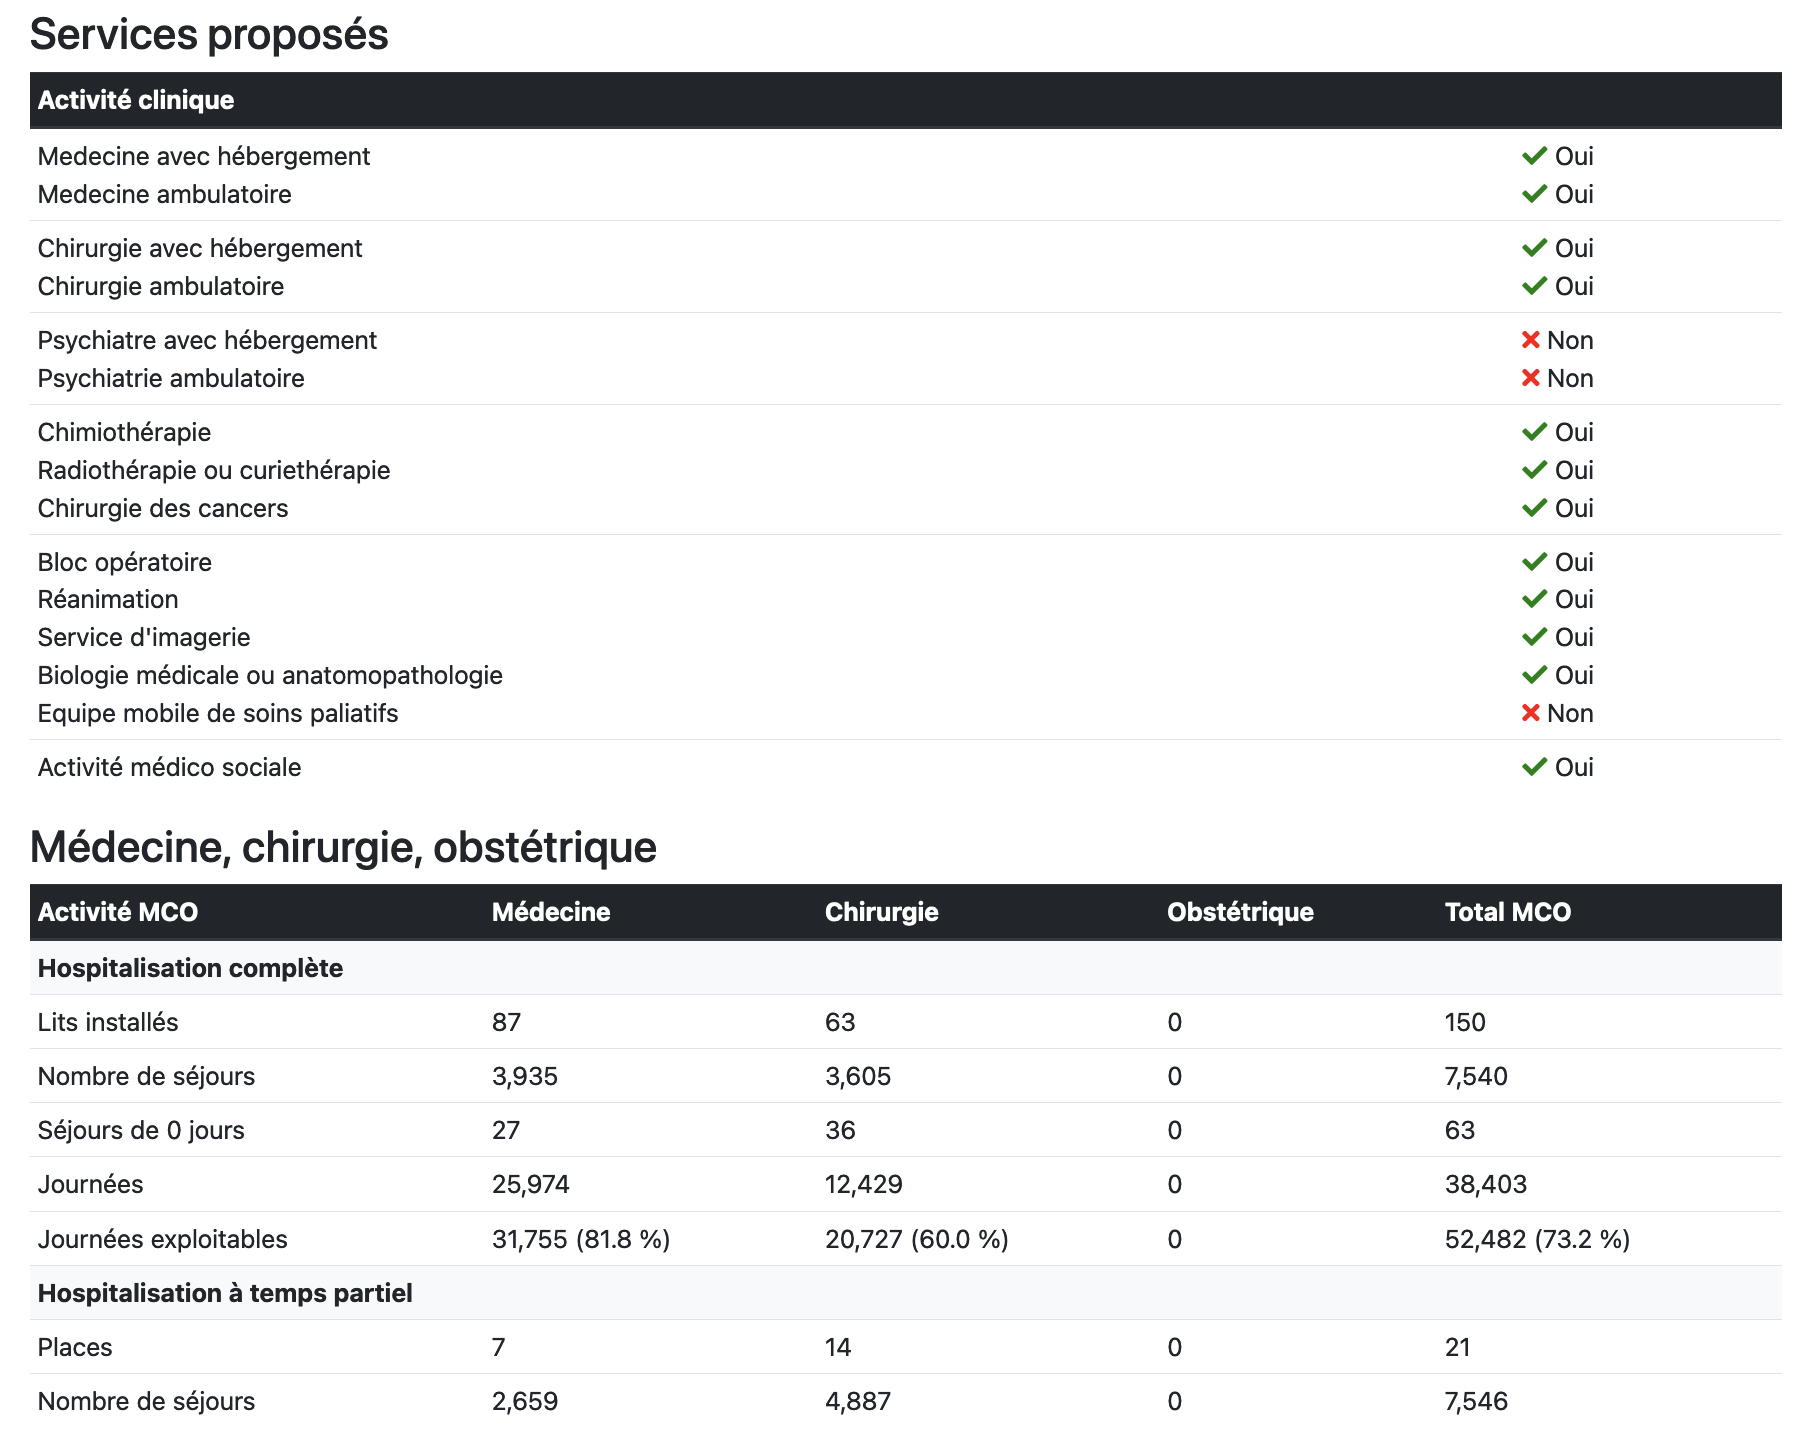
\includegraphics[width=0.7\textwidth]{images/healthcare-network/curie-services.png}
    \centering
    \caption{ \textbf{Healthcare-Network: description of health services
            offered, and statistics on \ac{mco} activity for Institut Curie Paris
            hospital.} The list of services allows to quickly evaluate the
        hospital ability to treat cancer patients. The number of stays and number of
        beds lets the users evaluate the hospital size, and how saturated it is.}
    \label{fig:hn-curie-services}
\end{figure}

Next, we display a section focused on oncology activity, we show statistics
related to cancer care, as illustrated on \cref{fig:hn-curie-cancero}. This
section lists the key oncology services like radiotherapy, cancer surgery and
chemotherapy authorization. The number of cancer related stays, the number of
radiotherapy stays as well as the number of beds dedicated to oncology are
shown.

\begin{figure}[h]
    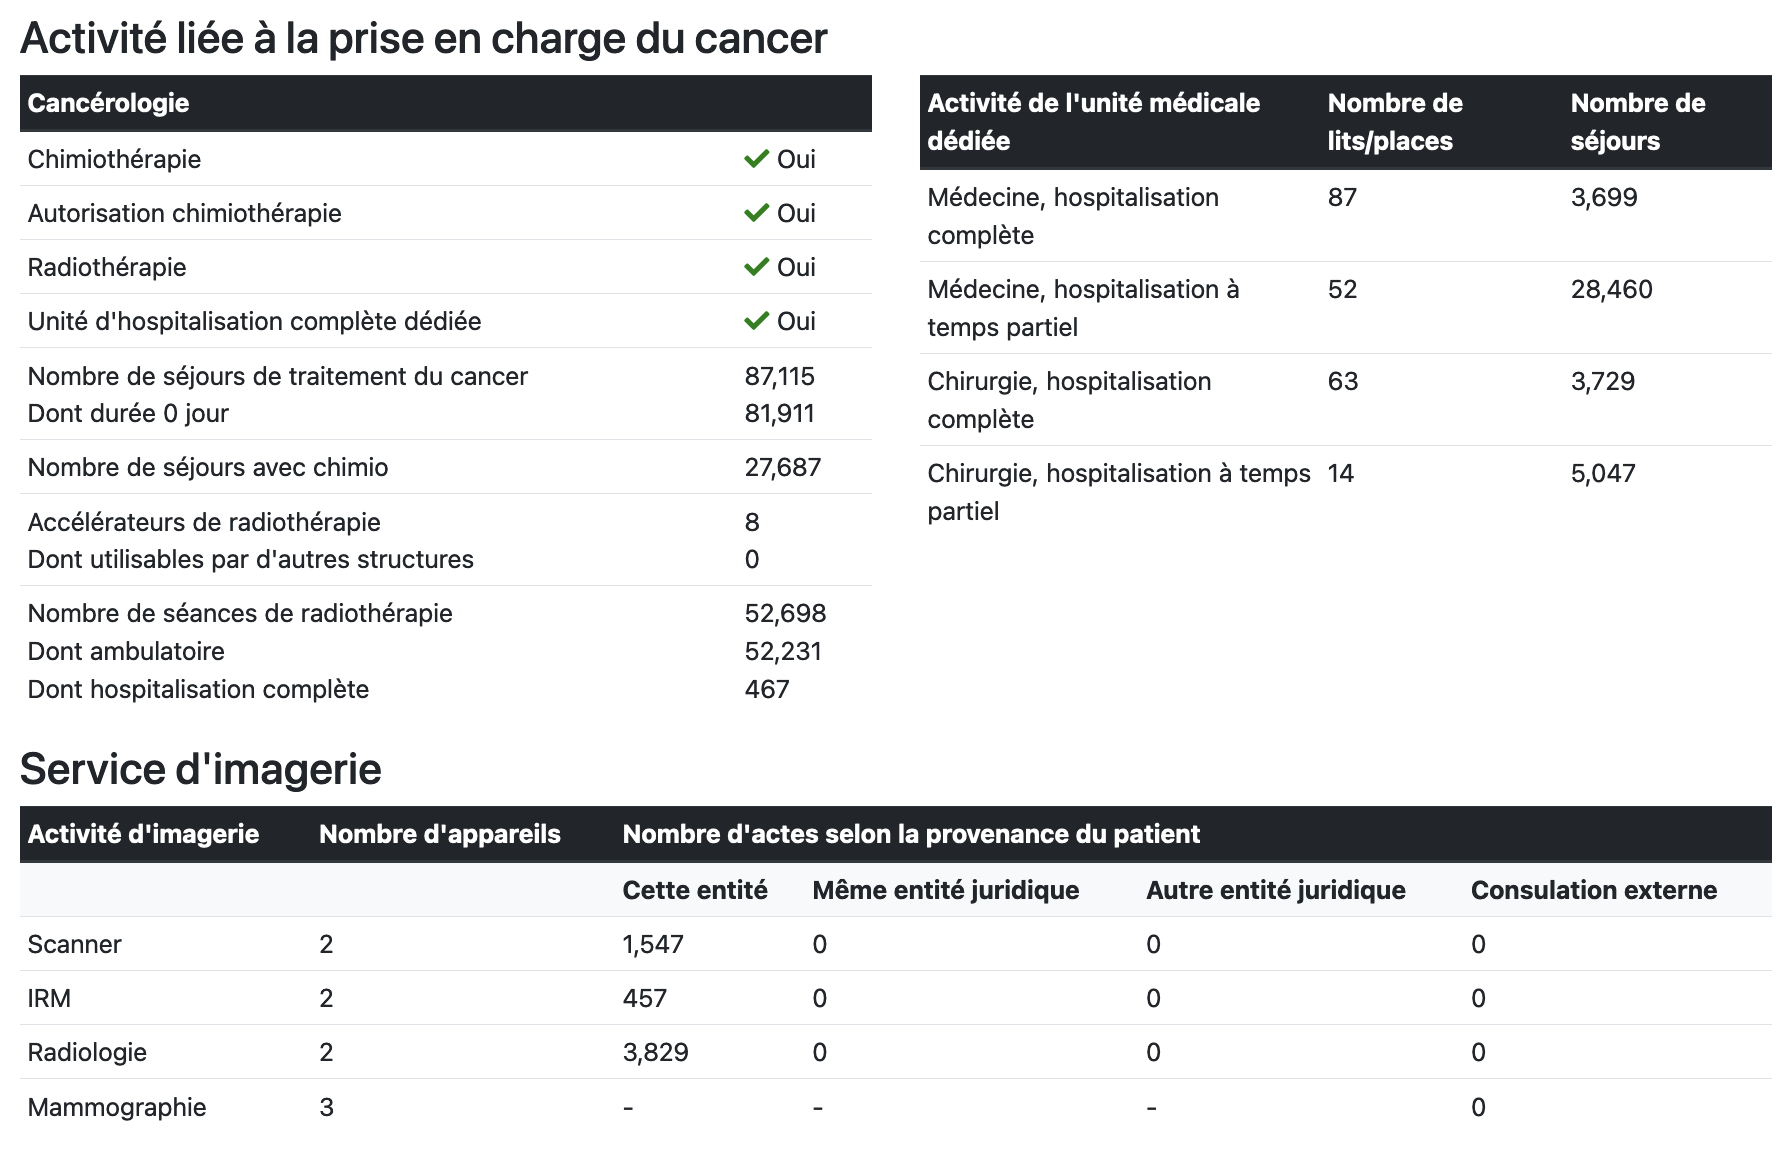
\includegraphics[width=0.7\textwidth]{images/healthcare-network/curie-cancero.png}
    \centering
    \caption{
        \textbf{Healthcare-Network: description of oncology activity for Institut Curie Paris hospital.}
    }
    \label{fig:hn-curie-cancero}
\end{figure}

Finally, we show the number of patients stays by cancer organs treated in the
hospital. We chose a radar chart visualization, as displayed on
\cref{fig:hn-curie-dp}. Three series are shown on this plot. First, in green, we
show the statistics of the current hospital. Then, in purple, we display the
median number of patients treated for every hospital in the same category, while
the orange curve shows the overall median. Showing these three variables allows
the users to compare the current hospital with hospitals within the same
category as well as broader comparison to the overall median. In this case, the
numbers are from Institut Curie hospital. The radar chart shows that this
hospital treats more patients than the other hospitals from the same category,
especially for eye cancer, where Institut Curie is among the only hospitals with
expertise on this rare cancer.

\begin{figure}[h]
    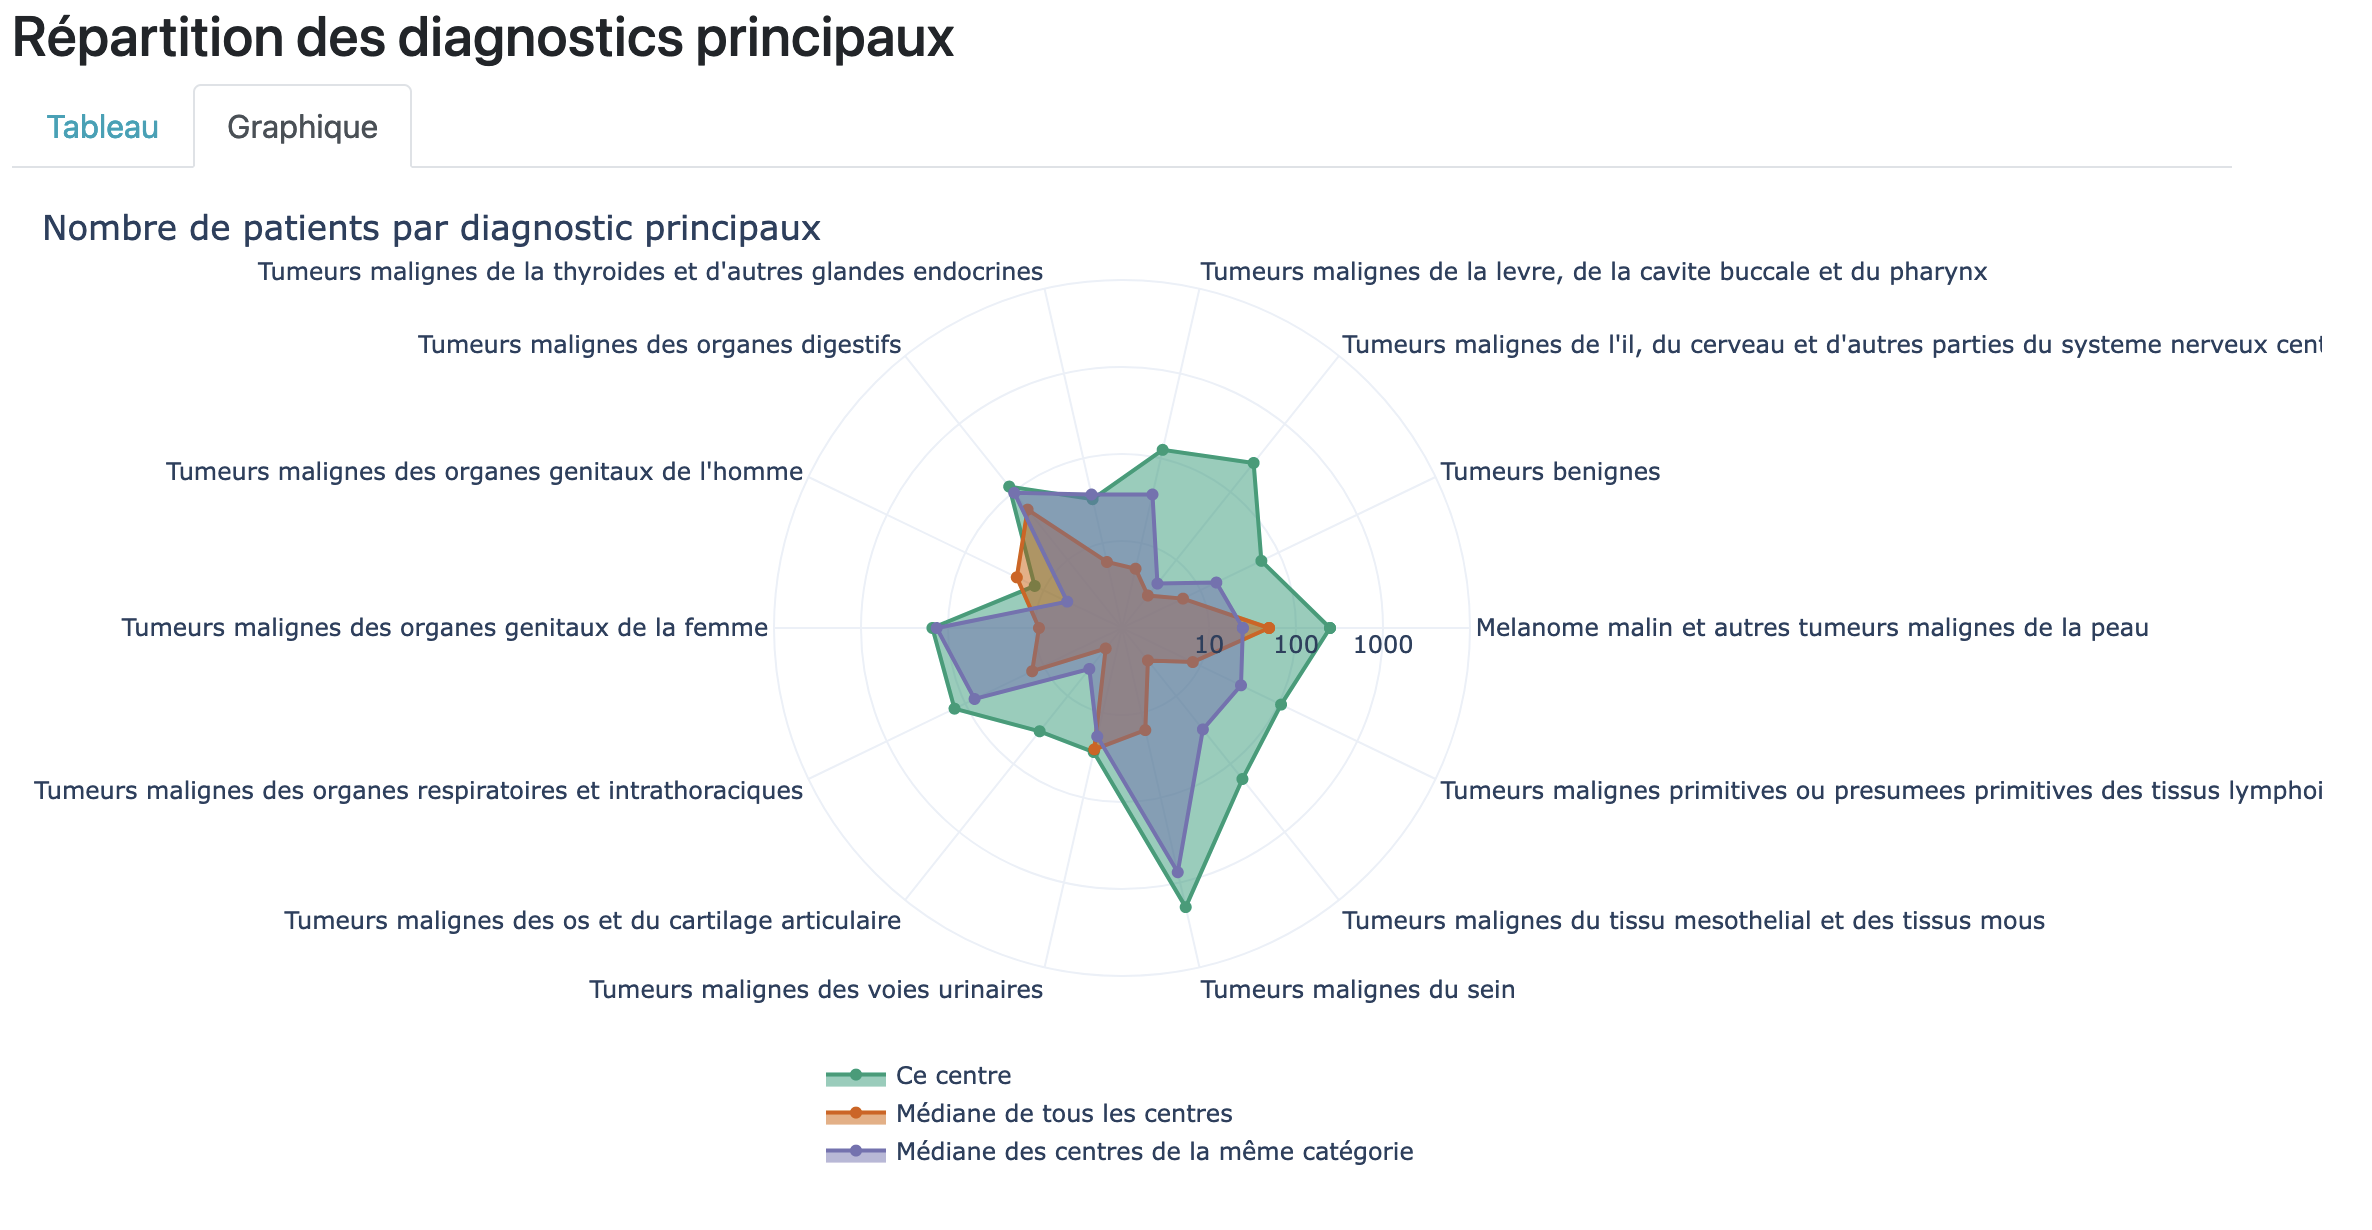
\includegraphics[width=0.7\textwidth]{images/healthcare-network/curie-dp.png}
    \centering
    \caption{ \textbf{Healthcare-Network: number of patients per cancer related
            diagnosis for Institut Curie Paris hospital.} Comparison with the median
        statistics from hospitals within the same category (\ac{clcc}) and
        overall median. }
    \label{fig:hn-curie-dp}
\end{figure}

To gain insights about the hospital neighborhood, we show socio-demographic
statistics on the municipality where the hospital is located. In the case of
Institut Curie, the municipality is the 5\textsuperscript{th} arrondissement of
Paris. Among the numbers displayed, we have the municipality size, population,
median salary and poverty rate. We also count the number of health professionals
by occupation within the hospital department, and within the hospital. This
gives information on the link between the hospital and the town medicine which
is very important for patient care.

\begin{figure}[h]
    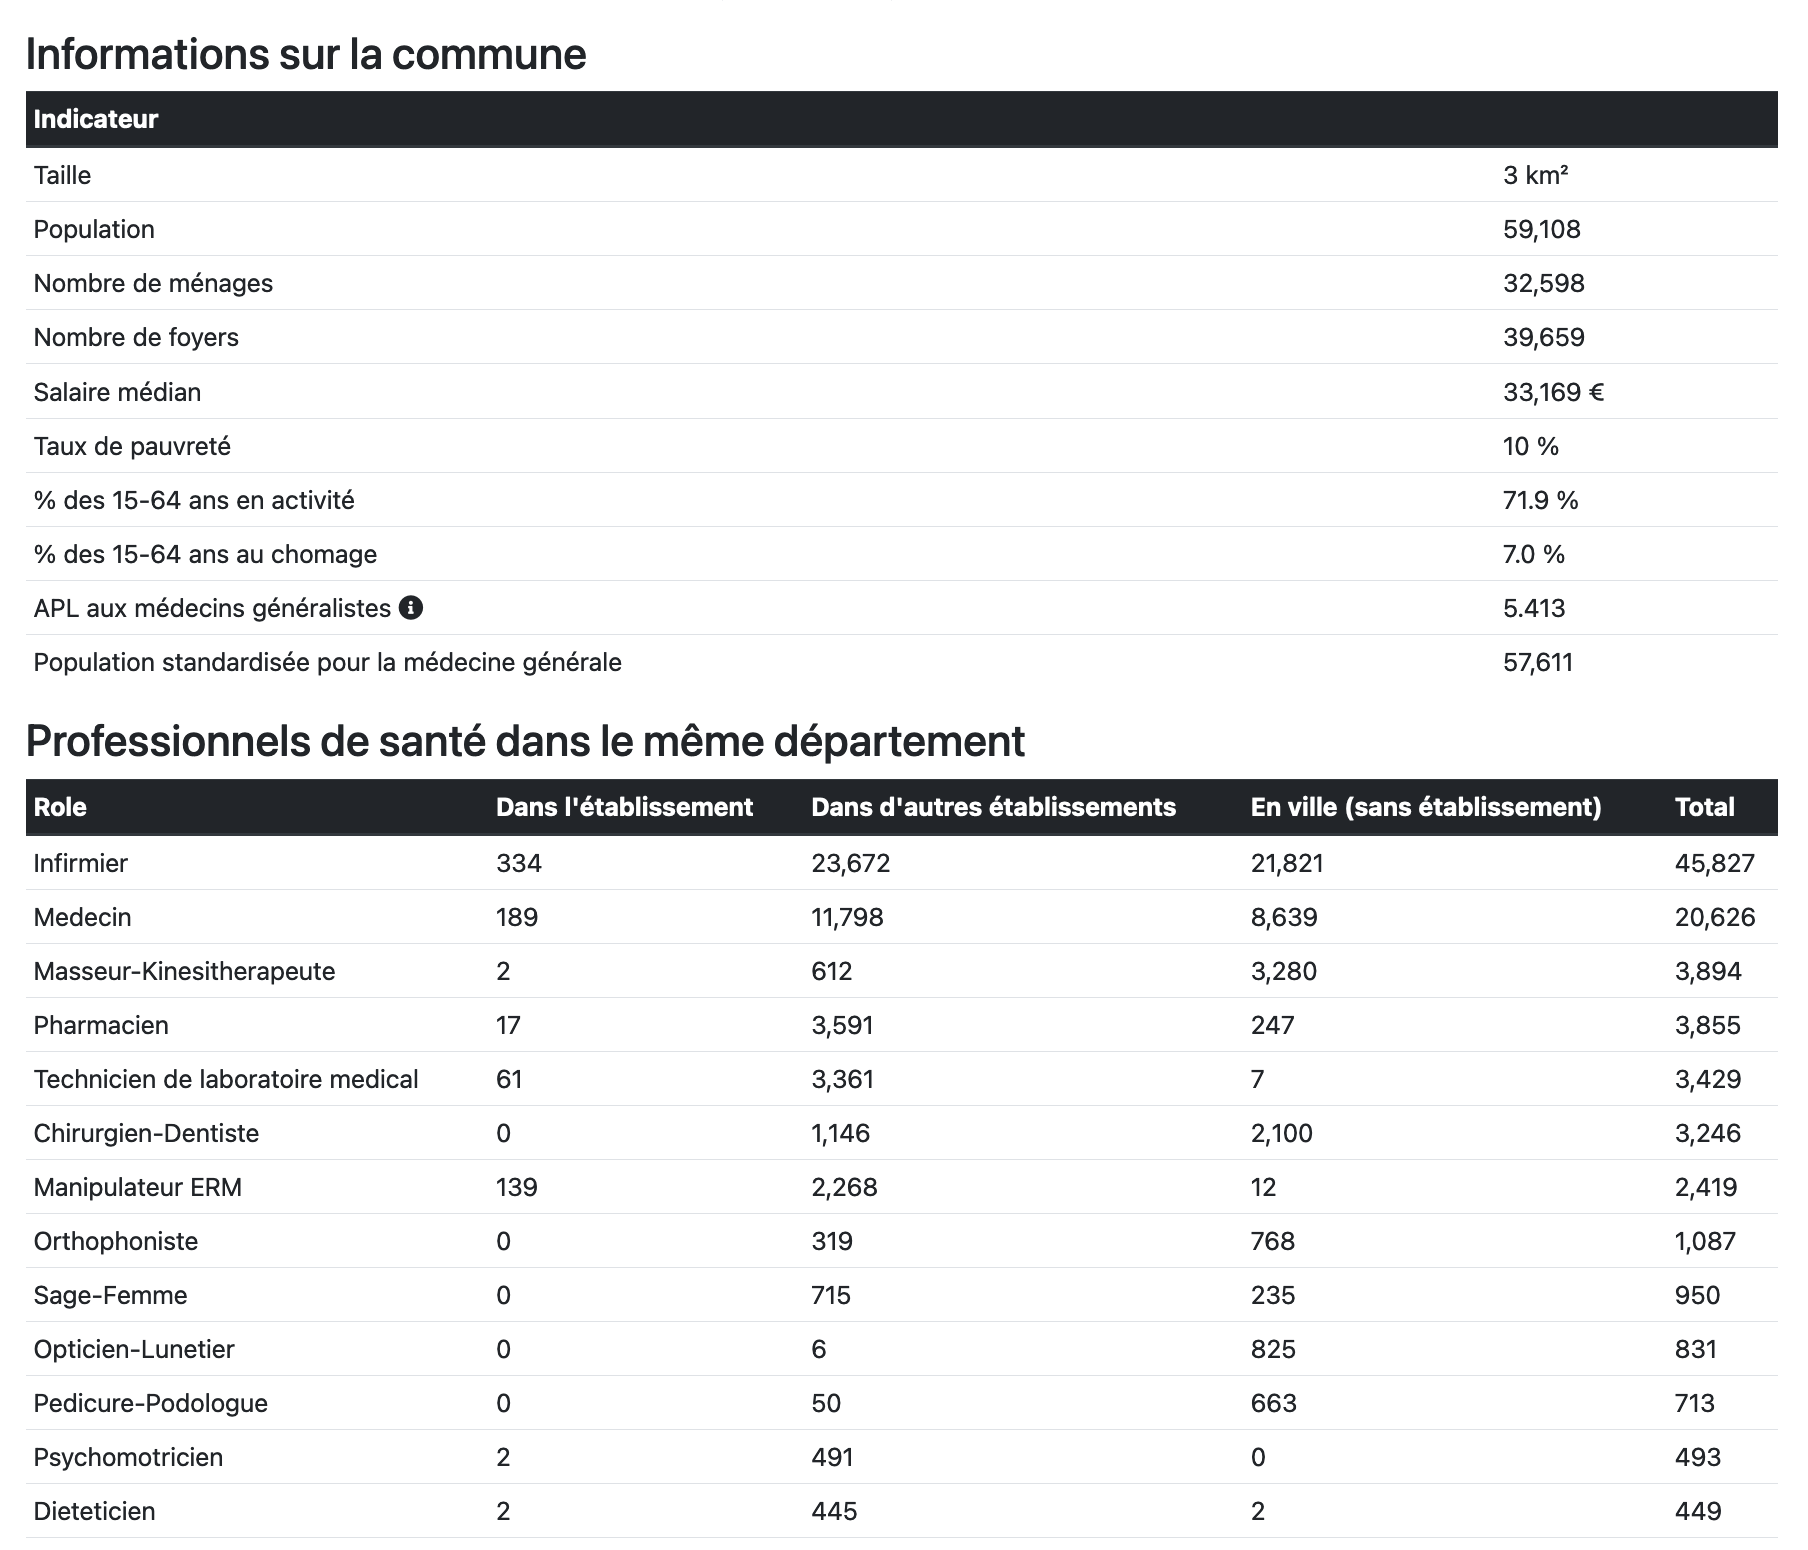
\includegraphics[width=0.7\textwidth]{images/healthcare-network/curie-commune.png}
    \centering
    \caption{ \textbf{Healthcare-Network: statistics on the municipality where
            Institut Curie Paris is located (Paris 75105).} Population, median
        salary and accessibility to primary care are displayed to qualify the
        hospital neighborhood. Health professionals within the department are
        also listed to illustrate the health supply available around the
        hospital. }
    \label{fig:hn-curie-commune}
\end{figure}

\section{Conclusion}

Our Healthcare-Network web application could benefit both patients and
healthcare professionals. It might incentive health professionals to find a
closer hospital from the patient location, lowering both travel burden as well
as \ac{co2} emissions. Also, patients will be able to double check where they
have been sent to, which could reduce dissatisfaction and health disparities. In
Healthcare-Network, hospitals statistics are displayed in the most transparent
way possible. This often involves showing plain numbers to patients or health
professionals, which might be confusing and unclear for some. More work might be
needed to make sure the web application is intuitive and brings useful
information to everyone. Moreover, while we developed the web application with
the help of medical experts, we did not gather patients' feedback yet. The app
design and features are thus likely to change in the future. While our web
application brings more health information to the patients, we should be
cautious about undesired effects of this approach. Indeed, research showed that
the increase in the amount of available medical information resulted in some
difficulties for patients when search-ing for suitable doctors
\cite{narducci_recommender_2015,hoens_reliable_2010}. This gap opened the need
for patient-doctor matchmaking, in which patients can find the right doctors
based on several criteria \cite{han_hybrid_2018}. Recommender systems are a
typical way to solve such problems. They have been integrated into online
retailers, streaming services, and social networks to facilitate users' item
selection process. Recently, these systems have been widely applied to the
healthcare domain to help both end-users and medical professionals in making
more efficient and accurate health related decisions
\cite{tran_recommender_2021}. Recommender systems have also been used to provide
personalized doctor recommendations based on emotions and preferences of users
about doctors through their ratings and reviews \cite{zhang_idoctor_2017}.
Although the current literature has shown many benefits of \ac{hrs} to improve
their health conditions, there still exist some gaps regarding developing and
evaluating \ac{hrs} that need to be bridged \cite{tran_recommender_2021},
especially during their evaluation \cite{calero_valdez_recommender_2016}.
Uncertainty in \ac{hrs} links to potential risks and imprecise predictions since
user preferences are not al-ways captured well. For these reasons, we chose not
to embed a hospital recommender system in the web application yet, since the
information we have on the patients are not detailed enough. Showing the health
facilities nearby the patients' location as well as some key statistics is a
good first step to assist patients and health professionals during the hospital
selection. Moreover, while mass media communications can be an important source
of health information, research found social disparities in health knowledge
that may be related to media use. Indeed, cancer-related health communications
seems to be patterned by race, ethnicity, language, and social class. The
benefits of health information are not equally distributed across socially
distinct groups in the United States \cite{viswanath_race_2011}. A lower
likelihood of cancer information seeking was also observed among those with
lower education levels, lower income and greater ages
\cite{finney_rutten_cancer-related_2016}. Therefore, we must make sure our tool
can be accessed by most of the patients, and efforts must be made in addressing
these social disparities. Improving healthcare by making it more connected will
not be sufficient as it will not benefit a non-insignificant part of the
population. The full benefits of a more connected and transparent healthcare
will show when the more deprived populations can access such tools.
